\chapter{Results and Conclusions}

%This section should discuss issues you encountered as you tried to implement your experiments. What were the results of running the experiments? What conclusions can you draw from these results?

%During the work, you might have found that elements of your experiments were unnecessary or overly complex; perhaps third party libraries were available that simplified some of the functions that you intended to implement. If things were easier in some areas, then how did you adapt your project to take account of your findings?

%It is more likely that things were more complex than you first thought. In particular, were there any problems or difficulties that you found during implementation that you had to address? Did such problems simply delay you or were they more significant?

%If you had multiple experiments to run, it may be sensible to discuss each experiment in separate sections.
\section{Results}

\begin{figure}[H]
  \centering
  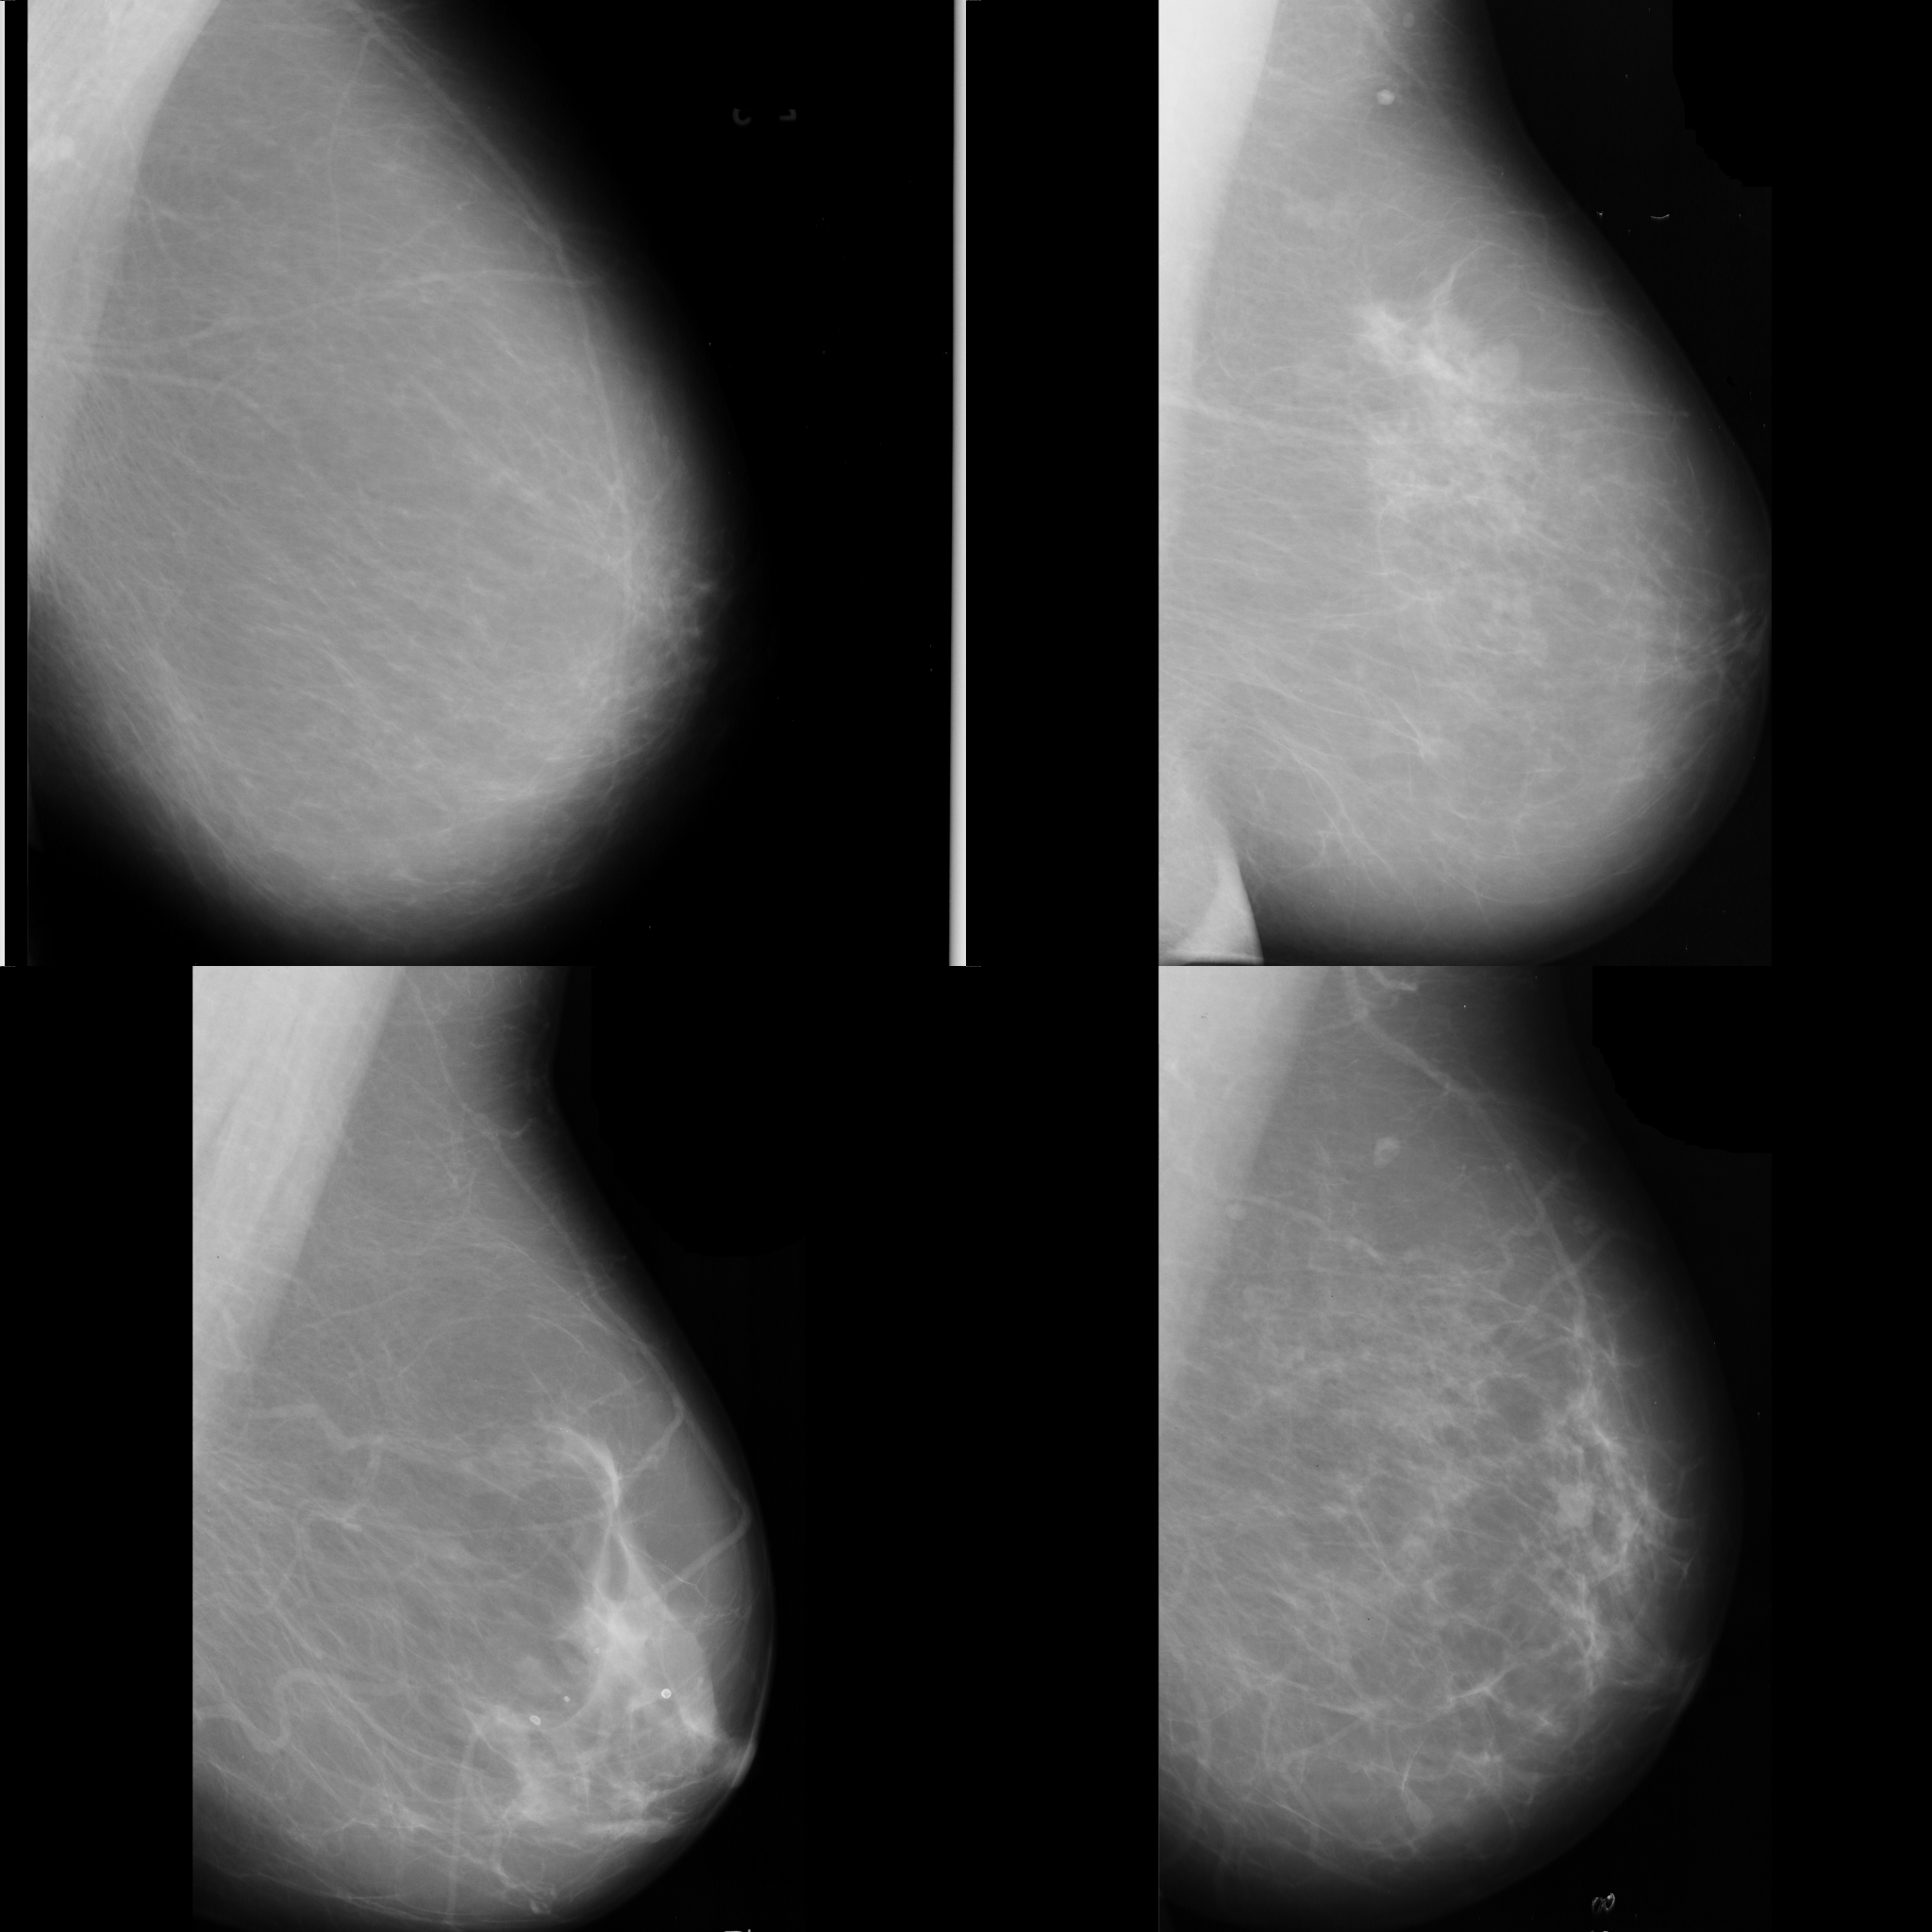
\includegraphics[width=0.4\textwidth]{Chapter3/results-img/big_scan.png}
  \caption{4 input scans.}
  \label{fig:input-data}
\end{figure}

% http://tex.stackexchange.com/questions/202072/scale-y-and-x-axis-in-pgfplots
\begin{figure}[H]
  \begin{center}
    \iffalse
    \begin{tikzpicture}
      \begin{axis}[
        width=15cm,
        axis lines = middle,
        scaled ticks=false,
        grid=both,
        ymin=0,ymax=0.7,
        xlabel=$x$,ylabel=$y$,
        ytick={0,0.1,...,1},
        xtick={0,...,20},
        xlabel={\large Iteration},
        ylabel={\large Entropy},
        legend entries={Hybrid entropy,Non-Probabilistic entropy,Shannon entropy},
         x label style={at={(axis description cs:0.5,-0.05)},anchor=north},
         y label style={at={(axis description cs:-0.05,.5)},rotate=90,anchor=south},
        ]
        \addplot table [x=Iteration, y=Entropy, col sep=comma] {Chapter3/hybrid-img/hybrid20.csv};
      \addplot table [x=Iteration, y=Entropy, col sep=comma] {Chapter3/nonProb-img/nonprob20.csv};
      \addplot table [x=Iteration, y=Entropy, col sep=comma] {Chapter3/shannon-img/shannon-20.csv};
    \end{axis}
    \end{tikzpicture}
    \fi
    \caption{Comparison of the reduction in entropy over iterations.}
  \end{center}
\end{figure}

\newpage
\subsection{Shannon Entropy}

\begin{figure}[H]
    \centering
    \begin{subfigure}[t]{0.3\textwidth}
        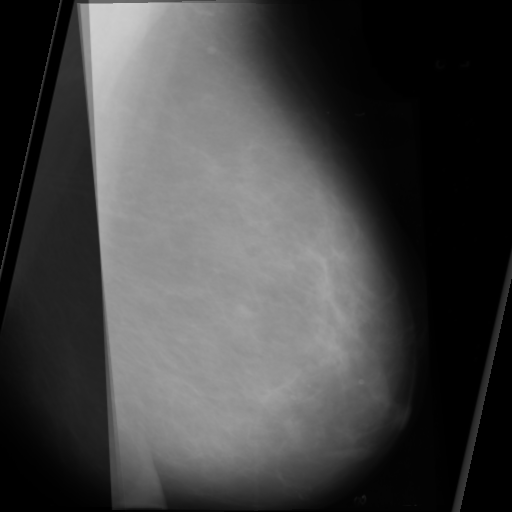
\includegraphics[width=\textwidth]{Chapter3/shannon-img/s-5-final.png}
        \caption{5 Shannon Entropy iterations.}
        \label{fig:5-shannon}
    \end{subfigure} \hfill
    ~ %add desired spacing between images, e. g. ~, \quad, \qquad, \hfill etc.
      %(or a blank line to force the subfigure onto a new line)
    \begin{subfigure}[t]{0.3\textwidth}
        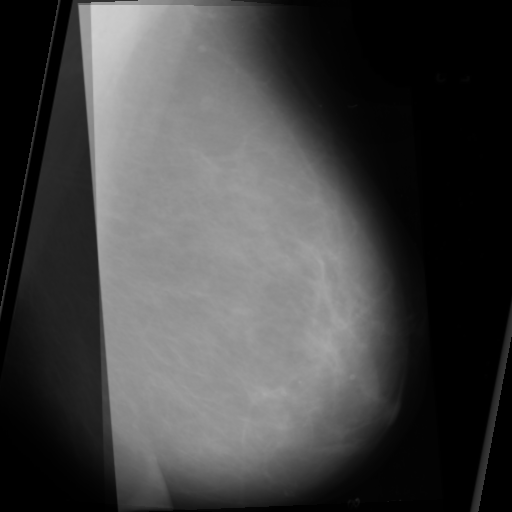
\includegraphics[width=\textwidth]{Chapter3/shannon-img/s-10-final.png}
        \caption{10 Shannon Entropy iterations.}
        \label{fig:10-shannon}
    \end{subfigure} \hfill
    \begin{subfigure}[t]{0.3\textwidth}
      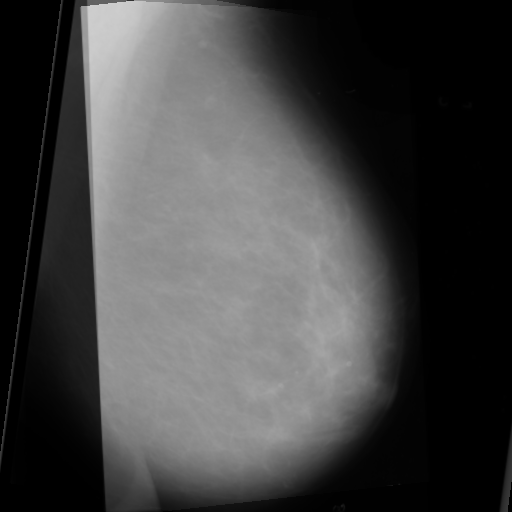
\includegraphics[width=\textwidth]{Chapter3/shannon-img/shannon-20.png}
      \caption{20 Shannon Entropy iterations.}
      \label{fig:20-shannon}
    \end{subfigure}
\end{figure}

\begin{figure}[H]
  \begin{center}
    \iffalse
    \begin{tikzpicture}
      \begin{axis}[
        width=12cm,
        axis lines = middle,
        scaled ticks=false,
        grid=both,
        ymin=0.5,ymax=0.6,
        xlabel=$x$,ylabel=$y$,
        xtick={0,...,20},
        xlabel={Iteration},
        ylabel={Entropy},
        legend entries={Shannon entropy},
        x label style={at={(axis description cs:0.5,-0.05)},anchor=north},
        y label style={at={(axis description cs:-0.1,.5)},rotate=90,anchor=south},
        ]
      \addplot table [x=Iteration, y=Entropy, col sep=comma] {Chapter3/shannon-img/shannon-20.csv};
    \end{axis}
    \end{tikzpicture}
    \fi
    \caption{Shannon: Comparison of the reduction in entropy over iterations, as in Table \ref{table:shannon-entropy}.}
  \end{center}
\end{figure}

\begin{table}
\pgfplotstabletypeset[col sep=comma,
     columns={Iteration,Entropy},columns/Entropy/.style={precision=6}
    ]{Chapter3/shannon-img/shannon-20.csv}
    \caption{Entropy table for Shannon}
    \label{table:shannon-entropy}
\end{table}

\newpage
\subsection{Non-Probabilistic Entropy}

\begin{figure}[H]
    \centering
    \begin{subfigure}[t]{0.3\textwidth}
        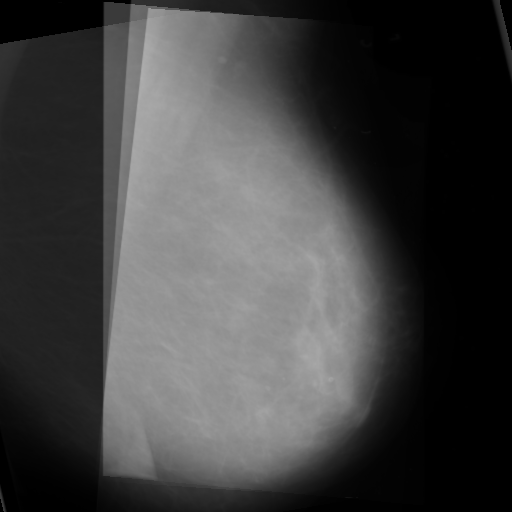
\includegraphics[width=\textwidth]{Chapter3/nonProb-img/nonProb-5.png}
        \caption{5 Non-Probabilistic entropy iterations.}
        \label{fig:5-nonProb}
    \end{subfigure} \hfill
    ~ %add desired spacing between images, e. g. ~, \quad, \qquad, \hfill etc.
      %(or a blank line to force the subfigure onto a new line)
    \begin{subfigure}[t]{0.3\textwidth}
      \includegraphics[width=\textwidth]{Chapter3/nonProb-img/nonProb10.png}
        \caption{10 Non-Probabilistic entropy iterations.}
        \label{fig:10-nonProb}
    \end{subfigure} \hfill
    \begin{subfigure}[t]{0.3\textwidth}
      \includegraphics[width=\textwidth]{Chapter3/nonProb-img/nonProb20.png}
      \caption{20 Non-Probabilistic entropy iterations}
      \label{fig:20-nonProb}
    \end{subfigure}
\end{figure}

\begin{figure}[H]
  \begin{center}
    \iffalse
    \begin{tikzpicture}
      \begin{axis}[
        width=12cm,
        axis lines = middle,
        scaled ticks=true,
        grid=both,
        xlabel=$x$,ylabel=$y$,
        xtick={0,...,20},
        xlabel={Iteration},
        ylabel={Entropy},
        legend entries={Non-Probabilistic entropy},
        x label style={at={(axis description cs:0.5,-0.05)},anchor=north},
        y label style={at={(axis description cs:-0.08,.5)},rotate=90,anchor=south},
        ]
      \addplot table [x=Iteration, y=Entropy, col sep=comma] {Chapter3/nonProb-img/nonProb20.csv};
    \end{axis}
    \end{tikzpicture}
    \fi
    \caption{Non-Probabilistic: Comparison of the reduction in entropy over iterations, as in Table \ref{table:non-prob-entropy}.}
  \end{center}
\end{figure}

\begin{table}
\pgfplotstabletypeset[col sep=comma,
     columns={Iteration,Entropy},columns/Entropy/.style={precision=6}
    ]{Chapter3/nonProb-img/nonProb20.csv}
    \caption{Entropy table for Non-Probabilistic}
    \label{table:non-prob-entropy}
\end{table}

\newpage
\subsection{Hybrid Entropy}

\begin{figure}[H]
    \centering
    \begin{subfigure}[t]{0.3\textwidth}
        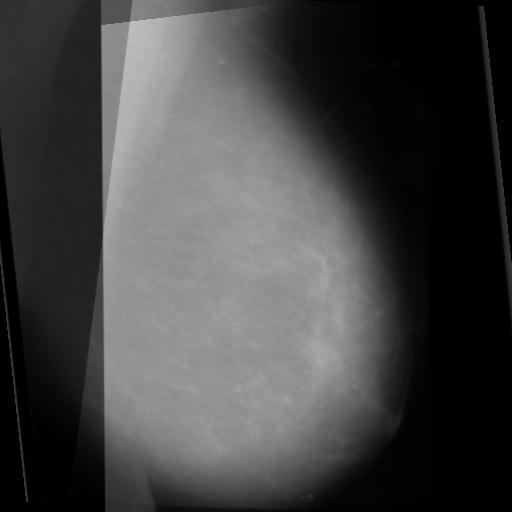
\includegraphics[width=\textwidth]{Chapter3/hybrid-img/hybrid-5.png}
        \caption{5 Hybrid entropy iterations.}
        \label{fig:5-hybrid}
    \end{subfigure} \hfill
    ~ %add desired spacing between images, e. g. ~, \quad, \qquad, \hfill etc.
      %(or a blank line to force the subfigure onto a new line)
    \begin{subfigure}[t]{0.3\textwidth}
      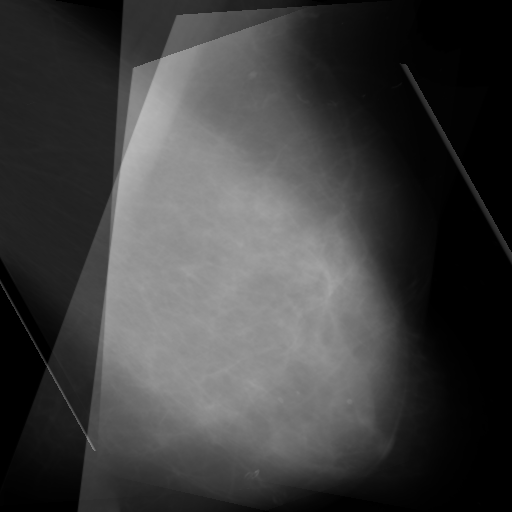
\includegraphics[width=\textwidth]{Chapter3/hybrid-img/hybrid-10.png}
        \caption{10 Hybrid entropy iterations.}
        \label{fig:10-hybrid}
    \end{subfigure} \hfill
    \begin{subfigure}[t]{0.3\textwidth}
      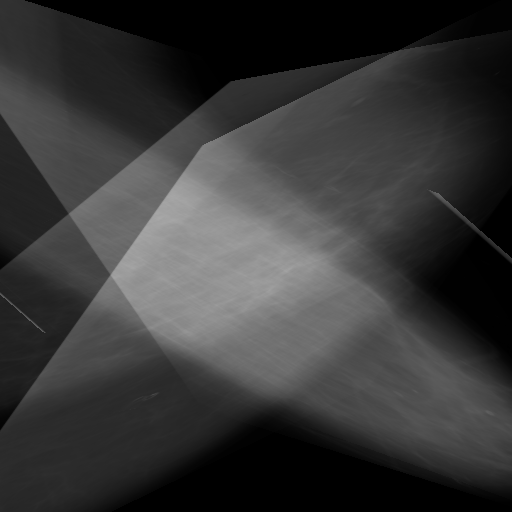
\includegraphics[width=\textwidth]{Chapter3/hybrid-img/hybrid20.png}
      \caption{20 Hybrid entropy iterations.}
      \label{fig:20-hybrid}
    \end{subfigure}
\end{figure}

\begin{figure}[H]
  \begin{center}
    \iffalse
    \begin{tikzpicture}
      \begin{axis}[
        width=12cm,
        axis lines = middle,
        scaled ticks=true,
        grid=both,
        xlabel=$x$,ylabel=$y$,
        xtick={0,...,20},
        ymin=0,ymax=0.3,
        xlabel={Iteration},
        ylabel={Entropy},
        legend entries={Hybrid entropy},
        x label style={at={(axis description cs:0.5,-0.05)},anchor=north},
        y label style={at={(axis description cs:-0.1,.5)},rotate=90,anchor=south},
        ]
      \addplot table [x=Iteration, y=Entropy, col sep=comma] {Chapter3/hybrid-img/hybrid20.csv};
    \end{axis}
    \end{tikzpicture}
    \fi
    \caption{Hybrid: Comparison of the reduction in entropy over iterations, as in Table \ref{table:non-prob-entropy}.}
  \end{center}
\end{figure}

\begin{table}
\pgfplotstabletypeset[col sep=comma,
     columns={Iteration,Entropy},columns/Entropy/.style={precision=6}
    ]{Chapter3/hybrid-img/hybrid20.csv}
    \caption{Entropy table for Hybrid}
    \label{table:hybrid-entropy}
\end{table}
